% act_d4_student.tex — Iskole: Student Workflow
\documentclass[a4paper,landscape]{article}
\usepackage[a4paper,landscape,top=1.8cm,bottom=1.2cm,left=1.2cm,right=1.2cm]{geometry}
\usepackage[dvipsnames,svgnames]{xcolor}
\usepackage{tikz}
\usetikzlibrary{shapes.geometric,arrows.meta,calc}
\usepackage{fancyhdr}
\definecolor{ColHdr} {RGB}{30,58,138}
\definecolor{ActFill}{RGB}{219,234,254}
\definecolor{ActLine}{RGB}{52,109,219}
\definecolor{SysFill}{RGB}{220,254,220}
\definecolor{SysLine}{RGB}{34,139,34}
\definecolor{SwimBg} {RGB}{240,240,248}
\tikzset{
  nd_start/.style={circle,fill=black,minimum size=10pt,inner sep=0pt},
  nd_stop/.style={circle,fill=black,draw=black,double,double distance=2pt,minimum size=10pt,inner sep=0pt},
  nd_act/.style={rectangle,rounded corners=3pt,draw=ActLine,fill=ActFill,text width=4.9cm,minimum height=0.62cm,align=center,font=\footnotesize},
  nd_sys/.style={rectangle,rounded corners=3pt,draw=SysLine,fill=SysFill,text width=4.9cm,minimum height=0.62cm,align=center,font=\footnotesize\itshape},
  arr/.style={-{Stealth[length=5pt,width=4pt]},thick},
}
\newcommand{\swimbox}[4]{%
  \fill[SwimBg,rounded corners=4pt](#1-2.6,#2+0.15) rectangle (#1+2.6,#3);
  \node[font=\small\bfseries\color{ColHdr}] at (#1,#2) {#4};}
\pagestyle{fancy}\fancyhf{}
\fancyhead[C]{\bfseries\color{ColHdr}Iskole — Activity Diagram 4: Student Workflow}
\fancyfoot[C]{\small\thepage}
\renewcommand{\headrulewidth}{1pt}
\renewcommand{\headrule}{\hbox to\headwidth{\color{ColHdr}\leaders\hrule height 1pt\hfill}}
\setlength{\headheight}{16pt}
\begin{document}
\begin{center}
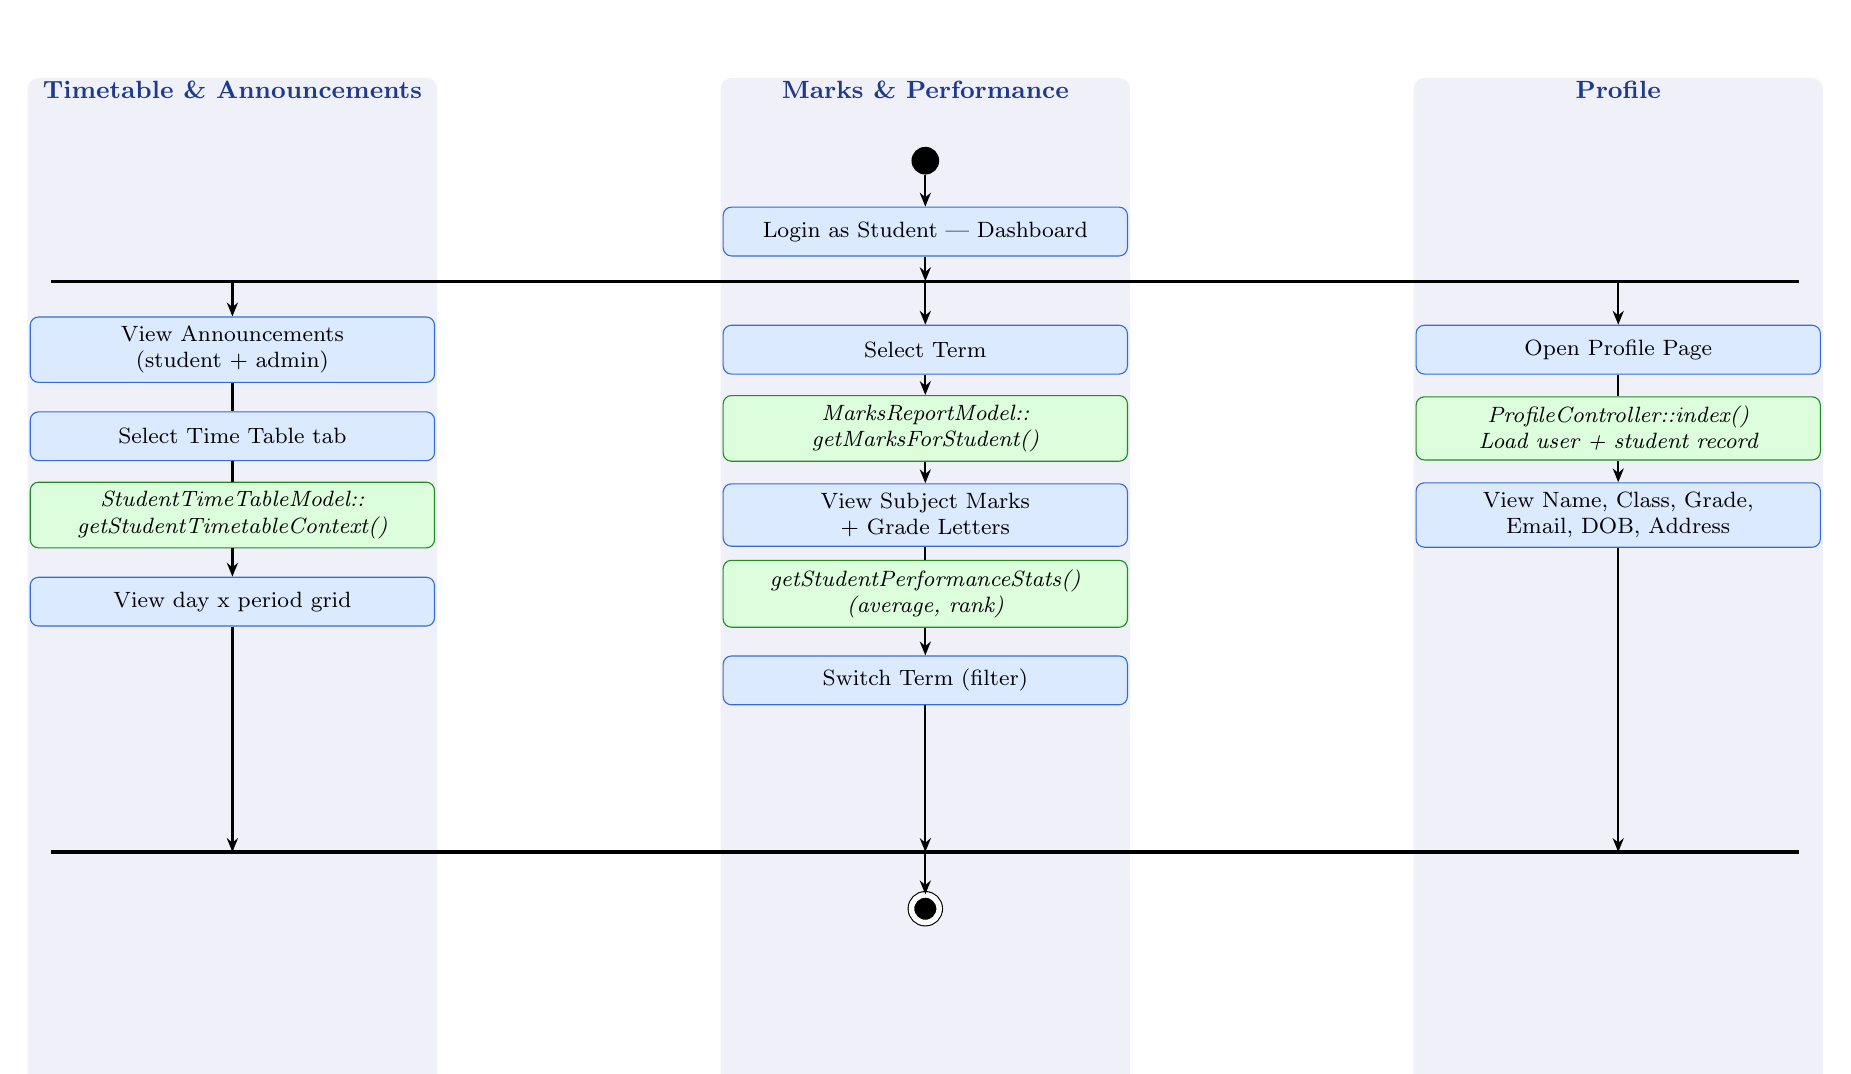
\begin{tikzpicture}[x=1cm,y=1cm]
\def\cA{4.5}\def\cB{13.3}\def\cC{22.1}
\swimbox{\cA}{0.2}{-12.5}{Timetable \& Announcements}
\swimbox{\cB}{0.2}{-12.5}{Marks \& Performance}
\swimbox{\cC}{0.2}{-12.5}{Profile}
\node[nd_start] at (13.3,-0.7)(S){};
\node[nd_act]   at (13.3,-1.6)(HD){Login as Student \textemdash{} Dashboard};
\fill[black](2.2,-2.25) rectangle (24.4,-2.21);
% Col A
\node[nd_act] at (\cA,-3.1)(A1){View Announcements\\(student + admin)};
\node[nd_act] at (\cA,-4.2)(A2){Select Time Table tab};
\node[nd_sys] at (\cA,-5.2)(A3){StudentTimeTableModel::\\getStudentTimetableContext()};
\node[nd_act] at (\cA,-6.3)(A4){View day x period grid};
% Col B
\node[nd_act] at (\cB,-3.1)(B1){Select Term};
\node[nd_sys] at (\cB,-4.1)(B2){MarksReportModel::\\getMarksForStudent()};
\node[nd_act] at (\cB,-5.2)(B3){View Subject Marks\\+ Grade Letters};
\node[nd_sys] at (\cB,-6.2)(B4){getStudentPerformanceStats()\\(average, rank)};
\node[nd_act] at (\cB,-7.3)(B5){Switch Term (filter)};
% Col C
\node[nd_act] at (\cC,-3.1)(C1){Open Profile Page};
\node[nd_sys] at (\cC,-4.1)(C2){ProfileController::index()\\Load user + student record};
\node[nd_act] at (\cC,-5.2)(C3){View Name, Class, Grade,\\Email, DOB, Address};
% join
\fill[black](2.2,-9.5) rectangle (24.4,-9.46);
\node[nd_stop] at (13.3,-10.2)(E){};
% arrows
\draw[arr](S)--(HD);
\draw[arr](HD.south)--(13.3,-2.23);
\foreach \x/\n in {\cA/A1,\cB/B1,\cC/C1}{\draw[arr](\x,-2.23)--(\n);}
\draw[arr](A1)--(A2)--(A3)--(A4);
\draw[arr](B1)--(B2);\draw[arr](B3)--(B4)--(B5);\draw[arr](B2)--(B3);
\draw[arr](C1)--(C2)--(C3);
\draw[arr](A4)--(\cA,-9.48);
\draw[arr](B5)--(\cB,-9.48);
\draw[arr](C3)--(\cC,-9.48);
\draw[arr](13.3,-9.46)--(E);
\end{tikzpicture}
\end{center}
\end{document}
